\subsection{Risk Analysis}
\label{risk}
It is important to thoroughly examine the risks associated with the project. When a risk is uncovered it is possible to take precautionary measures to minimize possibility of the risk happening. It will also allow us to make plans for what to do if a risk should become reality. This section will describe these issues.

Table \ref{riskshort} shows the risks that we think can affect the project. 
We have evaluated what consequences these different risks could have to the project and the probability of them happening.
"Initiatives for consequences" describes what to do in order to lower the severity of the consequence.
"Initiatives for probability" explains what initiatives are taken to reduce the probability of the risk happening.
Estimating the cost for the different initiatives in the table is difficult, since most of them require meetings and follow up. 
This is labour that could have been spend on the project, so it has a value. 
To see an illustrative overview of all risks with their respective consequence and probability see figure \ref{cxp}.
The figure shows that risk C and G are very critical because of the high consequence and probability, therefore we need to maintain high focus on these risks. Generally risk with a high CxP value needs to be listed high on the agenda. 
Risk A and B are of less critical value and easier to solve without affecting the project much.

\def\arraystretch{1.7}
\begin{table}[h!]
\centering
\scriptsize
\begin{tabular}{|p{2.9cm} |p{0.4cm} |p{0.9cm} |p{0.9cm} |p{0.5cm} |p{3cm} |p{3cm} |p{0.7cm}|} 
\hline
Risk 	&	La\-bel	& Conse\-quence	& Prob\-ability	& CxP	& Initiatives \newline for consequence	& Initiatives \newline for probability	& Cost \\ \hline
Subcontractor let down & A & 3 & 1 & 3 & Have contact to a few different subcontractors & Continuous follow up on subcontractor & Time\\ \hline
Team member leaves     & B & 3 & 2 & 6 & Hire / find another team member & Status meetings to follow up on team members relation to the project & Time\\ \hline
Investment refused by investor/bank & C	& 5	&	4 & 20	& Several parts of the project have to be done in spare time & Present the project to more investors or banks. Develop a good business plan & Time\\  \hline
Delay in development & D & 3 & 3 & 9 & Deprioritise some features & Regularly review development plan and status & Time\\ \hline
Unable to sell product / cannot sell enough & E & 5 & 2 & 10 & Produce product on order & Prepared to adjust product price. Follow the market demand. & Less re-\newline venue\\ \hline
Unable to establish collaboration with robot welding company & F & 5 & 2 & 10 & Contact with several companies & Maintain regularly contact to companies  & Time \\ \hline
Competitor "steals" the market & G & 5 & 3 & 15 & Good product pitch & Track information about competitors & Time\\ \hline
\end{tabular}
\caption{Risks which are having an impact on the project}
\label{riskshort}
\end{table}
\def\arraystretch{1}


\begin{figure}[h!]
\centering
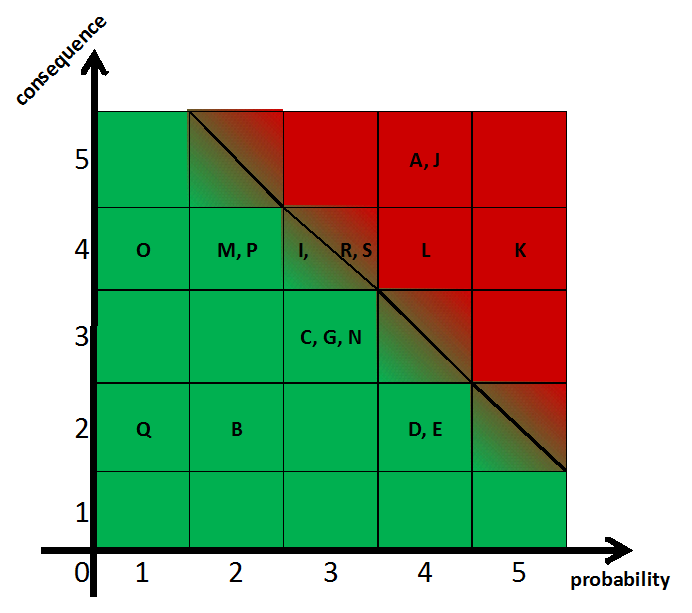
\includegraphics[scale=0.6]{./graphics/cxp}
\caption{Consequence and probability diagram with placed risks}
\label{cxp}
\end{figure}
